\documentclass[12pt, a4paper]{article}

\usepackage[utf8]{inputenc}
\usepackage[T1]{fontenc}
\usepackage[margin=2.5cm]{geometry}
\usepackage{graphicx}
\usepackage{hyperref}
\usepackage{parskip}
\usepackage{enumitem}
\usepackage{titlesec}
\usepackage{lmodern}

\newcommand{\eat}[1]{}
\newcommand{\HRule}{\rule{\linewidth}{0.5mm}}

\hypersetup{
    colorlinks=true,
    linkcolor=black,
    urlcolor=blue
}

\begin{document}

% Title page
\begin{titlepage}
\begin{center}

% Top 
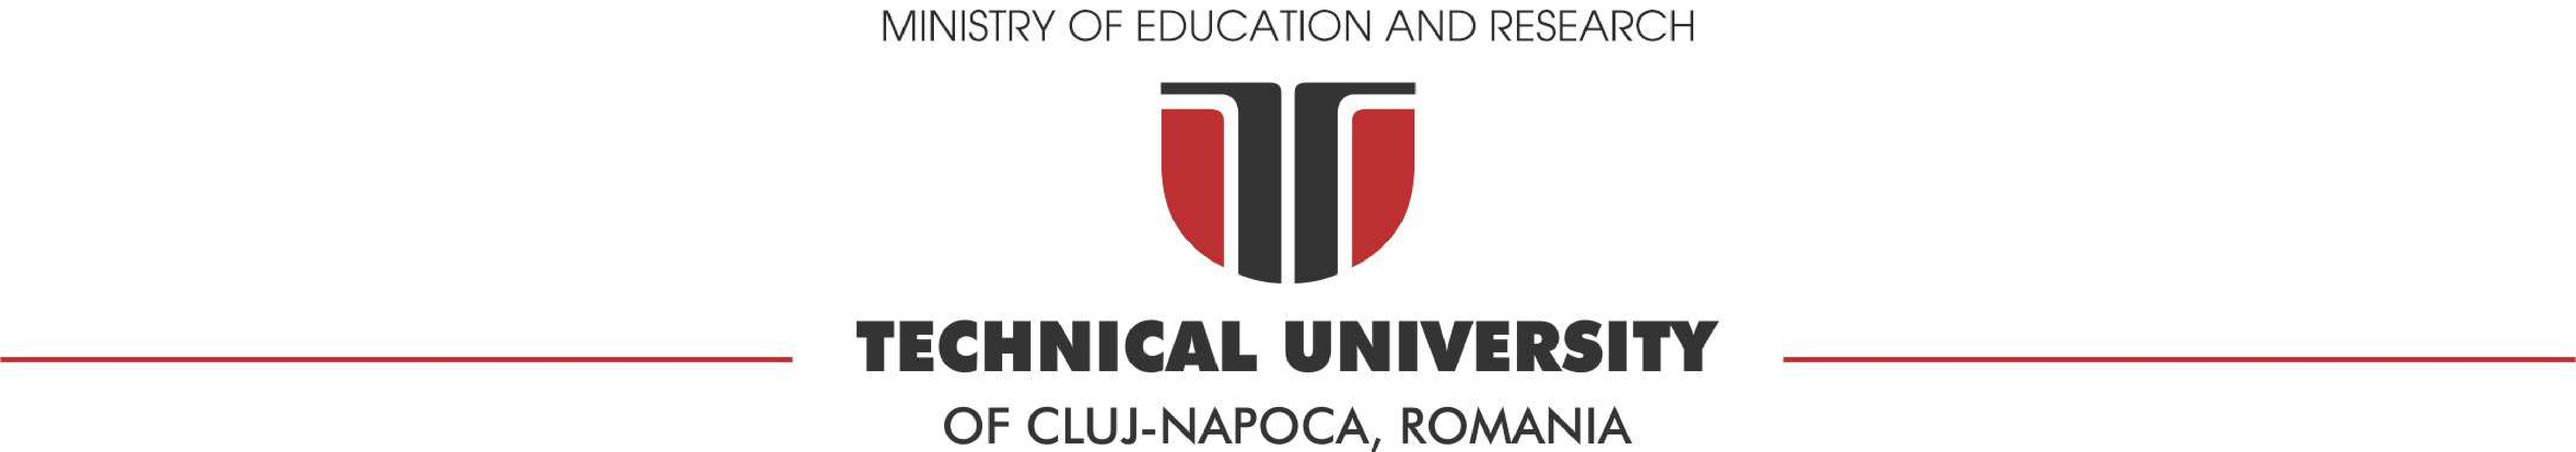
\includegraphics[width=1\textwidth]{AntetUTCNEng.pdf}~\\[2cm]

% Title
\HRule \\[0.4cm]
{ \LARGE
    \textbf{Project Assignment}\\[0.4cm]
    \emph{Software Design}\\[0.4cm]
}
\HRule \\[1.5cm]

% Author
{ \large \flushright
    Author: Varga Andrei\\[0.1cm]
    Group: 30433\\[0.1cm]
}

\vfill
\textsc{\large Faculty of Automation and Computer Science}\\[0.4cm]

% Bottom
{\large June 2026}
    
\end{center}
\end{titlepage}

\tableofcontents
\newpage

% -------------------------------------------------------
\section{Problem definition}

The goal of this project is to extend the online marketplace application built in the previous
assignments into a full client-server distributed system. The core domain remains unchanged: the
application manages users, shops, products and orders in an online marketplace context.

The new requirements for this assignment focus on separating the client from the server,
adding real-time communication through a chat feature, supporting multiple languages in the
interface, and handling errors in a consistent way across the whole system.

The analysis phase identifies the actors and use cases of the system. The design phase
describes the architecture, the data model and the key components. The implementation phase
covers the technology choices and the structure of the project. Finally, the testing section
describes the unit tests written to verify the business logic.

Deliverables for this assignment:
\begin{itemize}
    \item A branch on the GitHub repository containing the complete source code.
    \item This documentation.
    \item A pull request assigned to the course reviewer.
\end{itemize}

% -------------------------------------------------------
\section{Analysis phase - Use cases \& requirements}

\subsection{Functional requirements}

The system must support three user roles: Visitor, User, Store Manager and Administrator.
The main functional requirements are:

\begin{itemize}
    \item The system must allow visitors to browse the landing page and view public shop information.
    \item Users must be able to register and log in using a username and password.
    \item Authenticated users must be able to place orders and view their order history.
    \item Store Managers must be able to manage the inventory of their shop (add/remove products, update stock).
    \item Administrators must have full CRUD access to users, products, shops and orders.
    \item All authenticated users must have access to a real-time chat room.
    \item The interface must support switching between Romanian and English.
    \item The system must return structured error responses and display them in the UI.
\end{itemize}

\subsection{Use cases}

Below are the main use cases grouped by actor.

\textit{Visitor:} A visitor can see the landing page and browse existing shops. They can register
a new account or log in if they already have one.

\textit{User:} After logging in, a user can browse shops and products, place a new order by
selecting products with available stock, view their existing orders, and mark an order as paid.
They can also use the chat to communicate with other users.

\textit{Store Manager:} A store manager can view and manage their shop's inventory. They can
add new products to the shop with an initial stock, remove products, and increment or decrement
stock for existing ones. They also have access to the chat.

\textit{Administrator:} The administrator has access to all management pages. They can create,
update and delete users, products, shops and orders. They can also export the product list in
JSON, CSV or XML format.

\begin{figure}[h]
    \centering
    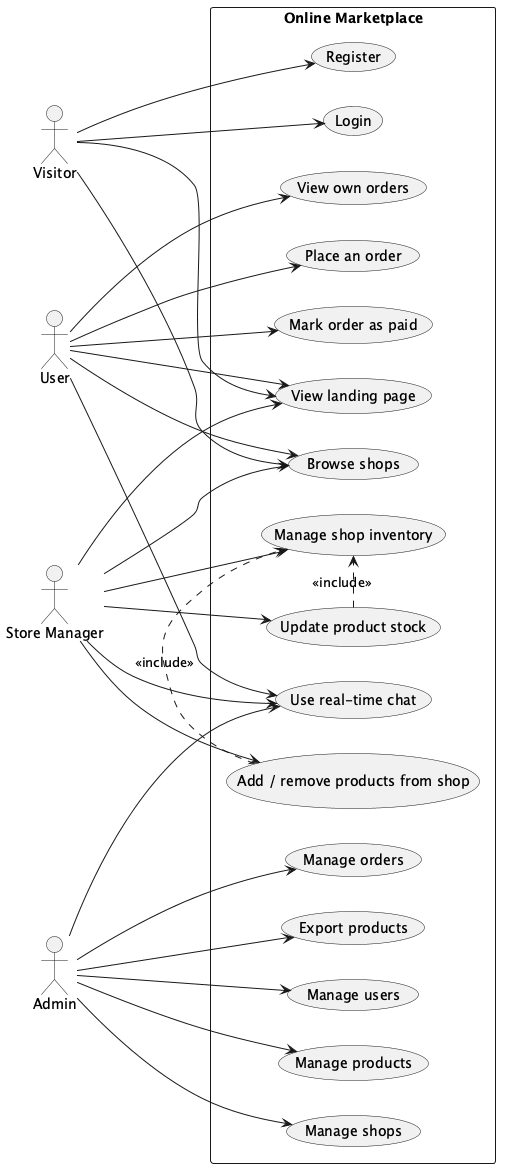
\includegraphics[width=0.9\textwidth]{use_case.png}
    \caption{Use case diagram}
    \label{fig:usecase}
\end{figure}

% -------------------------------------------------------
\section{Design phase}

\subsection{Architecture overview}

The system follows a microservices client-server architecture. The backend is split into six
independent services, each with its own database and a single responsibility. All traffic from
the browser goes through an nginx reverse proxy which routes requests to the appropriate
service based on the URL path.

The services are:
\begin{itemize}
    \item \texttt{users-service} --- handles registration, login and user management. Uses PostgreSQL.
    \item \texttt{products-service} --- manages product CRUD and export. Uses PostgreSQL.
    \item \texttt{shop-service} --- manages shop data and product stock. Uses PostgreSQL.
    \item \texttt{orders-service} --- manages order creation and lifecycle. Uses PostgreSQL.
    \item \texttt{notifications-service} --- listens to RabbitMQ events and sends email notifications. Uses MongoDB.
    \item \texttt{chat-service} --- provides a WebSocket endpoint for real-time messaging.
\end{itemize}

The frontend is a React + TypeScript single-page application built with Vite. It communicates
with the backend exclusively through the nginx proxy. JWT tokens are used for authentication:
the users-service issues a token on login, and the frontend attaches it to every subsequent
request via an axios interceptor.

The main advantage of this architecture is that each service can be developed, deployed and
scaled independently. The main downside is the added operational complexity: services need to
be coordinated, and cross-service data access requires additional HTTP calls or messaging rather
than simple joins.

\subsection{Entity-relationship diagram}

The data model is split across the services. Each service owns its own tables.

The \texttt{users} table stores user accounts with a role field (USER, STORE\_MANAGER, ADMIN).

The \texttt{shops} table stores shop information. The \texttt{admin\_id} column references a user
by ID (no foreign key constraint across services). The \texttt{shop\_product\_stock} table is a
map from product IDs to stock quantities for each shop.

The \texttt{products} table stores product details. The \texttt{shop\_id} column is a logical
reference to the shop the product belongs to.

The \texttt{orders} table stores order headers. Each order belongs to a user (by \texttt{user\_id}).
The \texttt{order\_item} table holds the individual line items with quantity and price at the
time of purchase.

The \texttt{notifications} collection in MongoDB stores domain events received from RabbitMQ.

\begin{figure}[h]
    \centering
    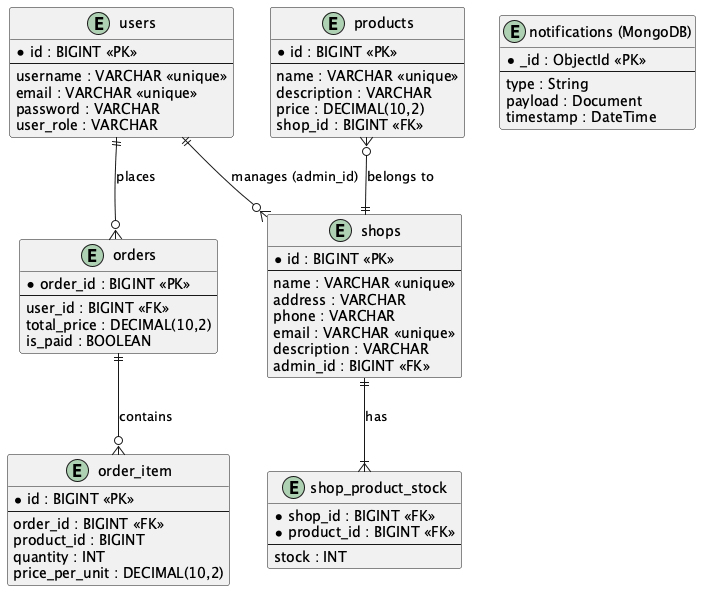
\includegraphics[width=0.9\textwidth]{er_diagram.png}
    \caption{Entity-relationship diagram}
    \label{fig:er}
\end{figure}

\subsection{Backend services}

Each backend service is a Spring Boot 4 application following a layered structure: controllers,
services, repositories and models. The command-query separation pattern is used consistently:
query controllers handle read operations and command controllers handle writes.

Every write operation in the backend is wrapped in a Command object following the Command
design pattern. A \texttt{CommandInvoker} executes these commands. This decouples the controller
from the business logic and makes it easy to add undo support or logging at the invoker level.

The \texttt{notifications-service} acts as an event consumer. When a product is created or an
order is placed, the responsible service publishes a message to RabbitMQ. The
notifications-service picks it up and sends an email to the user.

\subsection{Frontend}

The frontend is a React single-page application. Pages are protected by role: a
\texttt{ProtectedRoute} component checks the decoded JWT token stored in localStorage and
redirects to the landing page if the user does not have the required role.

All API calls go through a central axios instance defined in \texttt{src/api/client.ts}. This
instance has two interceptors: one that attaches the JWT token to every outgoing request, and
one that catches error responses and shows a browser alert with the message returned by the
server.

Internationalization is handled with \texttt{react-i18next}. Language files for English and
Romanian are stored in \texttt{src/locales/}. Users can switch languages from the navbar
and the preference is persisted in localStorage.

\subsection{Design patterns}

The following design patterns are used in the implementation:

\textit{Command pattern (behavioral)} --- used in all four backend services. Each write operation
(create, update, delete) is encapsulated in a Command class. The \texttt{CommandInvoker} runs
the command. This separates the request from its execution and makes the controller code thin.

\textit{Repository pattern (structural)} --- each service uses separate repository interfaces for
read and write operations (\texttt{IProductCommandService} / \texttt{IProductQueryService}), which
mirrors the CQRS concept.

\textit{Interceptor pattern (behavioral)} --- used on the frontend. The axios interceptors act as
middleware: the request interceptor adds the auth header, the response interceptor handles errors
uniformly so individual components do not need their own error handling logic.

\textit{Observer / Message broker pattern (behavioral)} --- the notifications-service subscribes
to RabbitMQ queues. Services that publish events do not need to know who consumes them, which
keeps the services loosely coupled.

\subsection{Class diagrams}

\begin{figure}[h]
    \centering
    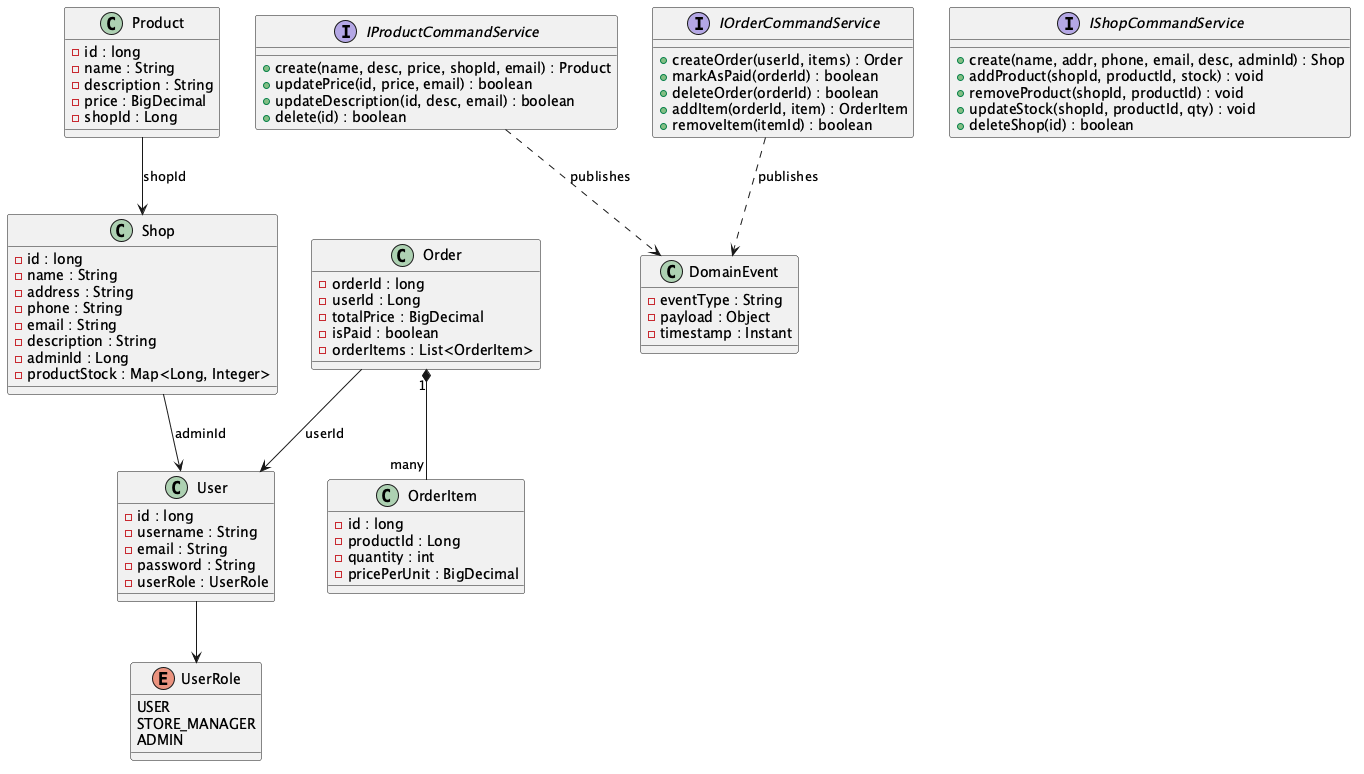
\includegraphics[width=0.95\textwidth]{class_diagram.png}
    \caption{Class diagram - core domain model}
    \label{fig:class}
\end{figure}

\subsection{Sequence diagrams}

The most important workflow is placing an order. The user opens the order form, the frontend
fetches available products and their stock levels, the user selects quantities, and the
frontend sends a POST request to the orders-service. The service saves the order and publishes
an event to RabbitMQ. The notifications-service receives the event and sends a confirmation
email to the user.

\begin{figure}[h]
    \centering
    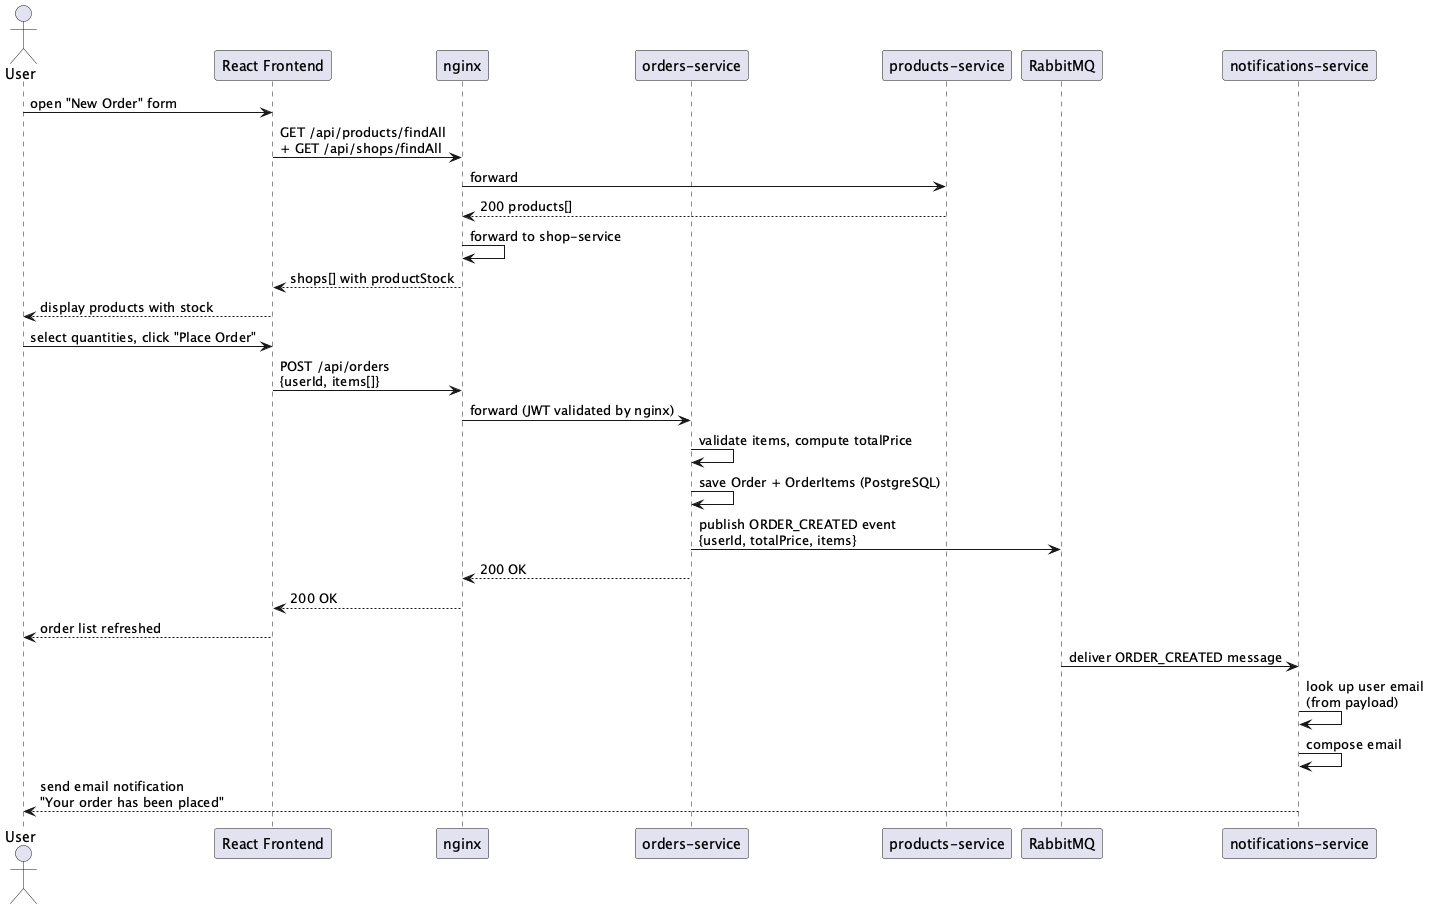
\includegraphics[width=0.95\textwidth]{sequence_diagram.png}
    \caption{Sequence diagram - placing an order}
    \label{fig:seq}
\end{figure}

% -------------------------------------------------------
\section{Implementation phase - Application}

\subsection{Tools and technologies}

\begin{itemize}
    \item Java 17 with Spring Boot 4 --- used for all backend services. Spring Web MVC handles
    REST endpoints, Spring Data JPA manages persistence, Spring Security provides JWT-based
    authentication in the users-service.

    \item PostgreSQL --- relational database used by users, products, shops and orders services.
    Each service has its own database to maintain independence.

    \item MongoDB --- used by the notifications-service to store event logs. A document database
    fits well here since the event payloads have variable structure.

    \item RabbitMQ --- message broker used to decouple services. The products and orders services
    publish events; the notifications-service consumes them.

    \item React 18 + TypeScript + Vite --- the frontend stack. Vite was chosen for fast
    development builds. TypeScript catches type errors early, which helps when working with
    multiple API response shapes.

    \item axios --- HTTP client for the frontend, chosen over fetch because interceptors are
    cleaner to implement for the centralized error handling and auth header injection.

    \item react-i18next --- internationalization library. Integrates well with React hooks and
    supports runtime language switching without a page reload.

    \item Docker + Docker Compose --- all services and infrastructure are containerized. This
    makes the setup reproducible and eliminates environment differences between machines.

    \item nginx --- reverse proxy that routes frontend requests to the correct backend service
    based on path prefixes (\texttt{/api/users}, \texttt{/api/products}, etc.) and handles
    WebSocket proxying for the chat service.

    \item JWT (jjwt 0.12) --- used for stateless authentication. The token encodes the username
    and role, which allows each service to verify requests independently without calling the
    users-service on every request.
\end{itemize}

\subsection{Application structure}

The repository is organized as a monorepo with one folder per service plus a \texttt{frontend}
folder and a root \texttt{docker-compose.yml}.

Each backend service follows the same internal structure:
\begin{itemize}
    \item \texttt{controller/} --- REST controllers (split into command and query controllers)
    \item \texttt{service/} --- business logic interfaces and implementations
    \item \texttt{repository/} --- Spring Data JPA repositories
    \item \texttt{model/} --- JPA entities
    \item \texttt{command/} --- command objects and invoker
    \item \texttt{dto/} --- request/response DTOs
    \item \texttt{config/} --- Spring configuration (CORS, RabbitMQ, security)
\end{itemize}

The frontend is organized as:
\begin{itemize}
    \item \texttt{src/pages/} --- one component per route
    \item \texttt{src/api/} --- axios wrappers for each service, plus the central client
    \item \texttt{src/components/} --- shared UI components (Navbar, ProtectedRoute, LanguageSwitcher)
    \item \texttt{src/locales/} --- translation files
    \item \texttt{src/utils/} --- auth helpers (JWT decode, localStorage access)
\end{itemize}

\subsection{User manual}

When opening the application, a visitor sees the landing page with general information.
They can navigate to the login page and authenticate. After login the navbar updates to show
the options available for their role.

A regular user sees links to their orders and the chat. On the orders page they can
create a new order by selecting products with available stock and entering quantities. The
total is calculated in real time. After placing the order they receive an email confirmation.

A store manager sees their shop's inventory and can add new products, adjust stock, or
remove products. They can also browse all shops.

An administrator has access to all management pages. On the products page they can filter
by price range, sort by name or price, and export the full list in JSON, CSV or XML. On the
orders page they can expand each order to see its line items.

The chat is available to all logged-in users. Messages are sent in real time over a WebSocket
connection and appear immediately for all connected users without refreshing the page.

The language switcher in the navbar lets users toggle between English and Romanian. The
preference is saved and restored on the next visit.

% -------------------------------------------------------
\section{Testing and validation}

Unit tests are written with JUnit 5 and Mockito and cover the service layer of the backend
services. The repository dependencies are mocked so the tests are fast and do not require
a running database.

For the products-service, the tests in \texttt{ProductCommandServiceTest} verify:
\begin{itemize}
    \item Creating a product calls the repository's \texttt{save} method and returns the saved entity.
    \item Updating the price of an existing product calls \texttt{updatePrice} on the repository and returns true.
    \item Updating the price of a product that does not exist returns false and does not call the repository.
    \item The same logic is tested for description updates and deletion.
\end{itemize}

Similar test classes exist for the orders-service (\texttt{OrderCommandServiceTest},
\texttt{OrderQueryServiceTest}), the shop-service (\texttt{ShopCommandServiceTest},
\texttt{ShopQueryServiceTest}) and the users-service (\texttt{UserCommandServiceTest},
\texttt{UserQueryServiceTest}).

The tests confirm that the service layer enforces the expected behavior independently of the
infrastructure. For example, operations on non-existent entities return false or throw
appropriate exceptions without causing unhandled errors in the controller.

\end{document}
